\section{Problem (3)}

	In the instant of the \cref{fig:hwb_problem3}, two particles move in an $xy$ plane. Particle $P_{1}$ has mass $1.8 \ sl$ and speed $v_{1} = \ 5.2 \ ft/s$, and it is at distance $d_{1} = \ 4.0 \ ft$ from point $O$. Particle $P_{2}$ has mass $1.2 \ sl$ and speed $v_{2} = \ 7.6 \ ft/s$, and it is at distance $d_{2} = \ 7.5 \ ft$ from point $O$. What is the net angular momentum of the two particles about $O$? Take counterclockwise as the positive direction.

	\begin{figure}[H]
		\begin{center}
			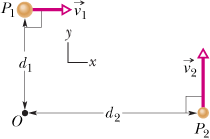
\includegraphics[scale=1]{hwb_problem3}
			\caption{Illustration of Problem 3}
			\label{fig:hwb_problem3}
		\end{center}
	\end{figure}

	\textbf{R:}

	\begin{align}
		L_{P_{1}} = \ &d_{1\perp}m_{1}v_{1}& \notag \\
		= \ &-(4.0 \ ft)(1.8 \ sl)(5.2 \ ft/s)& \notag \\
		= \ &- 37.44 \ sl \times ft^{2}/s& \notag \\
		L_{P_{2}} = \ &d_{2\perp}m_{2}v_{2}& \notag \\
		= \ &(7.5 \ ft)(1.2 \ sl)(7.6 \ ft/s)& \notag \\
		= \ &68.40 \ sl \times ft^{2}/s& \notag \\
		L_{net} = \ &L_{P_{1}} + L_{P_{2}}& \notag \\
		= \ &(- 37.44 \ sl \times ft^{2}/s) + (68.40 \ sl \times ft^{2}/s)& \notag \\
		= \ &30.96 \ sl \times ft^{2}/s&
	\end{align}
